\documentclass[11pt,a4paper,notitlepage,openany]{report}
\usepackage{floatrow}
\usepackage[pdftex]{graphicx}
\usepackage[hyphens]{url}
\usepackage[super,comma]{natbib}
\usepackage{listings}
\usepackage{minted}
\usepackage{multicol}
\usepackage{datetime}
\newdateformat{mydate}{\THEDAY\ \monthname[\THEMONTH] \THEYEAR}
\usepackage{csquotes}
\usepackage[linktoc=all]{hyperref}
\usepackage{changepage}
\usepackage{xcolor, colortbl}
\usepackage{tabu}
\usepackage{pdfpages}
\usepackage{amsmath}
\usepackage{pgfplots}
\usepackage[justification=centering]{caption}
\usepackage[titletoc,title]{appendix}
\usepackage{lscape}
\usepackage{geometry}
\usepackage{titling}
\usepackage{algorithm}
\usepackage{algpseudocode}
\usepackage{dirtytalk}
\usepackage{todonotes}
\usepackage{pifont}
\usepackage{titlesec}
\newfloatcommand{capbtabbox}{table}[][\FBwidth]
\usepackage{array}

% Useful custom commands which make text look better
%
% Issue by \<NAME> i.e. \hdfs
%
\usepackage{relsize}
\usepackage{xspace}
\newcommand{\post}{\textsmaller{POST}\xspace}
\newcommand{\tcpdump}{\textsmaller{TCPDUMP}\xspace}
\newcommand{\sslsplit}{\textsmaller{SSL}split\xspace}
\newcommand*\rot{\rotatebox{90}}
\newcommand*\OK{\ding{51}}
\algtext*{EndIf}% Remove "end if" text

\definecolor{butter1}{rgb}{0.988,0.914,0.310}
\definecolor{chocolate1}{rgb}{0.914,0.725,0.431}
\definecolor{chameleon1}{rgb}{0.541,0.886,0.204}
\definecolor{skyblue1}{rgb}{0.447,0.624,0.812}
\definecolor{plum1}{rgb}{0.678,0.498,0.659}
\definecolor{scarletred1}{rgb}{0.937,0.161,0.161}
\pgfplotsset{compat=newest}

\titleformat{\chapter}[display]
{\normalfont\huge\bfseries}{\chaptertitlename\ \thechapter}{20pt}{\Huge}
\titlespacing*{\chapter}{0pt}{5pt}{20pt}

\begin{document}
\begin{titlingpage}
\noindent
\begin{center}
\textsc{\Large Universiteit van Amsterdam}\\[0.2cm]
\textsc{\large System and Network Engineering}\\[0.5cm]

{ \large \bfseries Research Project 2}\\[0.2cm]
{ \LARGE \bfseries Session based high bandwidth throughput testing}\\[0.5cm]
\begin{footnotesize}
Bram ter Borch\\
\texttt{bram.terborch@os3.nl}\\[0.5cm]
{\large \mydate\today}
\end{footnotesize}

\centering
\vspace{1.0cm}

\includegraphics[scale=0.06]{images/uva_logo.png}
\vspace*{1.5cm}
\begin{abstract}
To maximize and ensure service availability, system and network administrators need to know what the limits of the infrastructure supporting a service are.
That infrastructure often has to support multiple different services for users and systems, the combined application demand placed on the infrastructure can result in parts of that infrastructure reaching its (practical) limit.
Generating packets in order to test the full capacity of a link is not hard to accomplish. 
Especially for UDP traffic since it does not provide session synchronization nor congestion control and does not offer retransmission of data. 
TCP, due to its design and used techniques, prevent the capacity of a network link or path from being overloaded. 

This research however focuses on the testing of limits pertaining to the packets per second rate and the number of concurrent sessions
This research investigates the suitability of various load testing tools - with and without the use of the Data Plane Development Kit - and apply these tools to various end-to-end network topologies and hardware systems that connect a client and a destination. 
The result of this research is a set of proposed tests, making use of the most suitable tools, to test an infrastructure up to application level. 
By using these proposed tests the report demonstrates that the weakest links in the path can be identified and its load tolerance limits can be found.

\end{abstract}
\end{center}
\end{titlingpage}

\renewcommand{\contentsname}{Table of Contents}
\setcounter{tocdepth}{1}
\tableofcontents
\addtocontents{toc}{\protect\enlargethispage{45mm}}
\begin{flushleft}
\end{flushleft}
\section{Introduction}
One hundred gigabit per second. In the world we live in this is a link speed you can get from you Internet Service Provider (ISP). When a business uses a link of 100Gb/s the security devices connected to this link also needs to be able to handle the traffic and apply security policies at least at this speed. Vendors offer machines with these capabilities. When looking at the specs of some vendors the maximum traffic is always represented in the form of Inter Mix (IMIX) traffic \cite{internetmix_2017}.
  

\chapter{Scope}\label{ch:problem}

%Currently there is no way of testing the full chain of devices towards, and including an application to their limits, without spending a lot of money on dedicated commercial load testing products.
The availability of high capacity links going up to 100Gb/s require infrastructure providers to maintain high capacity core networks in order to provide the increasing need for bandwidth.
An institute like Nikhef transfers a large volume of data and requires a reliable data transfer between source and destination.

In order to guarantee system uptime and service availability, the limitations of the hardware and services need to be known.  
In order to find the limitations, testing up to the application layer (layer 7) using open source software is preferred. 
The engineers at Nikhef never had the ability to perform high bandwidth applications tests at OSI layer 7. 

This chapter presents the scope for the problem stated in chapter \ref{ch:intro}. 
The scope is applicable for corporate networks in order to set the requirements for a set of tests during the experimental phase in chapter \ref{ch:experiments}.  
The scope and the problem lead to the research question presented at the end of this chapter. 

\section{The reliability of TCP}\label{sec:sessionbased}
When sending data over UDP, data gets generated and transported to the destination without any form of transport reliability. 
If the destination UDP port is open the data will be forwarded to the application listening on that specific port.
When the destination does not listen on that specific UDP port the data will be dropped.
The protocol does not provide feedback for any of the actions taken at the receivers side (except for ICMP error messages).
 
TCP, in contrast to UDP, guarantees the delivery of the data as long as the session is established between the end nodes.
The session needs to be created before data can be exchanged. 
A three way handshake between source and destination is performed in order to synchronize TCP settings. 
Guaranteed delivery is realized by acknowledging received data and resending unacknowledged data. 
Other techniques like flow control, congestion control and fast retransmission of packets ensure that data is delivered in time and offered to the higher layer protocol in the correct order. 
These techniques all require resource reservation at the client and the server, and at stateful network devices along the path between client and server. 

The techniques implemented in TCP require buffers to store data until the data is acknowledged by the receiving end.
The buffer sizes are reserved by the Operating System (OS) per session and are negotiated during the three way handshake.  
When more new sessions are created than the number of sessions that get closed due to a time-out or by terminating the session, eventually server resources will be depleted.

When it comes to layer 7 protocols like HTTP, even more resources need to be reserved. HTTP sessions, HTTP state and application state need to be saved. 
HTTP requests need to be processed, a response needs to be generated and sent over the session to the user. Normally a web server will cache files that are requested for a specific time using up memory. Hosting a dynamic web page requires the web server to generate the page on request which makes the CPU utilization higher than just hosting static web content. 

\section{Assumptions and constraints}\label{sec:specifications}
In order to execute some experiments and interpret their results, specific technical constraints in the real world operating environment and several key implementation parameters are important for this research. The technical constraints are not specific for Nikhef. The research is looking at a set of constraints that is applicable in corporate networks in order to specify requirements for this research.

\paragraph{Overloading}\label{par:overload}\mbox{}\\
All the built in techniques used by TCP ensure an IP path will not be overloaded. 
In order to find the weakest link in the path from a client to a service, data should be sent using the expected maximum capacity of the devices in the path.
When client and server are connected with 40Gb/s interfaces one should sent data using the maximum capacity of the links.
This could result in overloading a device in the path, which immediately shows that the intermediate device is the weakest link.

When data can be sent at the link's full capacity, there might be other hardware limitation (maximum amount of packets per second or a maximum amount of session per second) in the path to the destination.
For network and systems administrators it is important to know these limitation for monitoring purposes.

\paragraph{Throughput}\label{par:throughput}\mbox{}\\
The increasing need for bandwidth requires high capacity links between clients and destination in order to minimize transfer times.
A link's throughput is the most significant characteristic for generating load. 
This research considers links with a capacity of 40Gb/s and up, as high bandwidth links.
Therefor considered tools need to be able generate at least 40Gb/s of throughput, this is the first requirement.  

%When using TCP the header causes 12 bytes more overhead in comparison to a UDP header (a UDP header is 8 bytes). But in return TCP offers techniques that will not overload a device. 

\paragraph{Frame size}\label{par:framesize}\mbox{}\\
Ethernet is used during this research, therefore all references to frame sizes are based on Ethernet standards\cite{ethernet_frame_2017} with IP and TCP headers included.
Due to collision detection the minimum payload inside an Ethernet frame is 46 bytes.
The Ethernet frame and the payload combined have a minimum size of 64 bytes, this does not include a 4 byte VLAN tag. 
A packet is always preceded by an 8 byte preamble.
A 12 byte Inter Frame Gap between frames is used to separate the frames. 
This makes a total of at least 88 bytes of data from the beginning of a packet to the beginning of a new packet. 
A representation of an Ethernet frame that is used in the report is given in figure \ref{fig:juniperethernetframe}. 

\begin{figure}[H]
  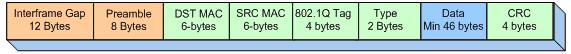
\includegraphics[scale=1]{images/ethernetframe.jpg}
  \caption{Representation of an Ethernet frame.}
  \label{fig:juniperethernetframe}
\end{figure}

\paragraph{Packet size}\label{par:packetsize}\mbox{}\\
According to Murray et all. \cite{murray2012state}  in 2012, 99\% of the traffic inside the corporate networks used during their research had an MTU size of maximum 1500 bytes. 
When using Jumbo frames\cite{alliance_2017} (best practice is an MTU of 9000 bytes towards clients\cite{jet}) the amount of overhead is less because more data can fit in one packet. 
More data inside a packet could result in less packets. 
Jumbo packets are helpful when large amounts of data need to be transfered between 2 nodes.  
Jumbo packets are not used during the project because according to Murray et all. less than one percent of transferred data has an MTU larger than 1500 bytes. 
Exceptions can be made during a test to see if hardware limits can be reached.

\paragraph{Packets per second}\label{par:pps}\mbox{}\\
When a link has a capacity of 40Gb/s and packets have a minimum size of 88bytes (which includes the inter frame gap, the preamble, the data link frame and a VLAN tag) a maximum of 56.8 million packets per second (Mpps) can be transferred over the link in one direction. When using a 100Gb/s line the theoretical maximum is 142 Mpps.   
The research is focusing on 40Gb/s links and therefore the second requirement is that a tool needs to be able to generate 56.8 million packets per second in order to be considered for the proposed tests.

\paragraph{Sessions}\label{par:sessions}\mbox{}\\
A TCP session is a unique tuple of source IP, destination IP, source port and destination port. 
An established session may be used to send more than one packet and can transfer data bidirectional.
The amount of sessions per second is a determining factor for the availability of services behind stateful devices. 
A stateful firewall, for example, needs to keep track of the states of the sessions from source to destination. 
When new sessions to a server are opened, the firewall has to process them according to the rule base. 
When a session is approved, most firewall vendors move it to fast-path processing. 
This is a table with accepted sessions, allowing traffic in the same session to be handled in hardware. This means that only the first packet of a new session is handled in the slow-path and the limitations of a firewall can be found in the amount of new sessions per second.
The amount of sessions the tool is capable of generating is the third requirement this research focuses on during the experimental phase.

\paragraph{Application specific traffic}\mbox{} \\
According to Sandvine\cite{phenomena_2017}, a global communications solutions service provider that published bi-annual traffic baseline reports, around 70\% of the traffic on the Internet is streaming audio and video. 
Dynamic Adaptive Streaming over HTTP (DASH)\cite{dash} is used to stream video and audio over HTTP. 
Netflix uses DASH to deliver content to the users. 
Next to DASH, streaming video services like YouTube are also accessible over HTTP.
Although the traffic inside the Nikhef network is not HTTP based, HTTP is the protocol that is the most used in the Internet. 
This makes HTTP a suited protocol to use for layer 7 tests during the research.  

\paragraph{End-to-end testing}\label{par:endtoend}\mbox{}\\
Performing tests by generating traffic between two connected links at OSI layer 2 or 3 does not test the limitations of an application. 
The application and the kernel should be tested using OSI layers above layer 4. 
When a server running an application is connected with a 40Gb/s link, it does not mean that the application can process 40Gb/s. 
End-to-end testing is a term used in this report to refer to tests that are application based.
A client sending application layer protocol requests and the server replying with application layer protocol responses.  

\section{Research question}\label{sec:researchquestion}
The problem statement and the specifications lead to the following research question.

\begin{center}
\textit{What are the requirements to perform high bandwidth session based throughput testing and how can this be applied to end-to-end application level testing?} \\
\end{center}


\chapter{Related Work}\label{ch:related}
As described in chapter \ref{ch:problem}, the goal of this research is the study of a reference model and an implementation for high bandwidth session and application based throughput testing.
Where the term "session based" refers to TCP sessions and the term "high bandwidth" refers to links of at least 40Gb/s.

\section{Transport layer protocols}
The project goal is to evaluate session-based high-throughput testing, which naturally leads to a focus on the session-oriented transport layer protocols. Similarly, UDP-based testing will not be used for the reference use cases and during the actual experiments.

\subsection{UDP}
When UDP traffic is generated, data is being dumped on the wire without keeping state nor resources need to be claimed for sessions on end hosts, except for the UDP send and receive buffers. 
Pktgen from the Linux kernel is an 'easy to use' application that is able to generate UDP-only traffic towards a destination. The destination does not need to run an application to receive the data.
The report written by Turull et al. \cite{turull2016pktgen} about pktgen is an updated report from their work in 2005 and looks at high speed networks. Where high speed for that report is everything over 10Gb/s.  

\subsection{TCP}
When TCP is used to transfer data, session states need to be kept by all the stateful hardware in the path from client to server. 
Congestion control starts to play a role at the senders end to make sure the intermediate devices will not be overloaded. 
The bandwidth filled by the client is dependent on the congestion control mechanism used by the sender.   
Emmerich et al. \cite{emmerich_gallenm¸ller_raumer_wohlfart_carle_2015} published a paper about MoonGen in 2015, MoonGen is capable of generating 120Gb/s and 178.5 Mpps (over multiple 10Gb ethernet interfaces using twelve 2 GHz CPU cores) according to the developers.
Exceeding the criteria for bandwidth and being session-based, it thus meets the requirements for this study.
Therefore, MoonGen looks like a good candidate for OSI layer 2, 3 and 4 testing. 

\subsection{Application specific}
In 2016 research was performed by Malakshmi et al. \cite{mahalakshmi2016study} on different DPDK applications with the purpose of creating a tool for L4 to L7 application testing. 
The result of Malakshmi's research is a tool called T-REX. Their projects goal is to generate stateful traffic up to 10Gb/s. 
However, the main T-REX functionality is Cisco-proprietary and requires a Cisco device to run. The public (free) version is limited in functionality to an extent that it is not interesting for this report.
\section{Tools}\label{sec:tools}
A lot of 'easy to use' tools are available for bandwidth testing. These tools each address one or more of the requirements for this study.
Specifically, we consider the tools listed in table \ref{table:tools} in order to assess the suitability of these tools for session based bandwidth testing at high volumes.
Pktgen kernel is capable of generating UDP packets only, it is used to determine differences in operating system characteristics for traffic generation. 
The biggest differences based on kernel behavior became evident based on tests with Pktgen kernel module.
Two different operating systems where used to see if different kernels provided different results. FreeBSD and Ubuntu supported all of the 'easy to use' kernel tools.

\begin{table*}[ht]
\centering
\begin{tabular}{|c|c|c|} \hline
\textbf{Tool} & \textbf{Session based} & \textbf{depends on} \\ \hline
iPerf3\cite{iperf} & Yes & Kernel  \\ \hline
hping\cite{hping}  & Yes & Kernel \\ \hline
BoNeSi\cite{bonesi} & Yes & Kernel \\ \hline
pktgen kernel\cite{pktgen-kernel} & No & Kernel \\ \hline
pktgen DPDK\cite{pktgen-dpdk} & Yes & DPDK \\ \hline
MoonGen\cite{moongen} & Yes & DPDK \\ \hline
WARP\cite{warp} & Yes & DPDK \\ \hline
\end{tabular}
\caption{Tested tools}
\label{table:tools}
\end{table*} 

\subsection{iPerf3}\label{sub:iperf3}
IPerf3 is a client-server based tool that allows packet generation.
IPerf3 is an improved version of iPerf that makes it possible the send traffic at higher rates than its predecessors. It needs a client and server to generate traffic and it needs tweaking of kernel parameter to generate traffic over 40Gb/s. Efforts have been made to make it available for DPDK \cite{jelte}. Unfortunately these efforts did not have the success the author was hoping for. 
A small test is performed to see if the kernel based version of iPerf3 can be used to generate high bandwidth session based traffic streams. The test and the results can be found in chapter \ref{ch:experiments}.

\subsection{hping}\label{sub:hping}
Hping was started in 2006. It is a command-line oriented TCP/IP packet assembler. Hping is capable of sending crafted packets to a destination using spoofed IP addresses if necessary. ICMP, UDP, TCP and RAW IP modes are supported. Random source addresses can be used to send requests to simulate a DDOS attack.    

\subsection{BoNeSi}\label{sub:bonesi}
BoNeSi is 'the DDOS botnet simulator' according to its developers. BoNeSi supports ICMP, UDP and TCP (HTTP) flooding attacks from a defined botnet size. Source addresses can be specified in a text file which is used as input. By doing this, one becomes capable of sending crafted packets from different source addresses.  

\subsection{pktgen(kernel module)}\label{sub:pktgenkernel}
To generate a single flow of UDP traffic without the need of an application at the other side, pktgen from the Linux kernel is the way to go. During the test phase preceding this paper, pktgen was tested on an Ubuntu machine and on a FreeBSD machine. 
This was done to see if there where any major differences at the kernel level that offer more bandwidth or more packets per second. 
As it turned out, FreeBSD has the ability to generate 40 million packets per second (pps) from one single thread. Ubuntu needs 6 threads to reach the maximum pps on a 40 Gb link. 
Other major differences where not found during this research between the different kernels. Therefore the FreeBSD kernel was abandoned after one week. 
Pktgen (kernel module) is only capable of generating UDP traffic and therefore, not usable for this research. 

\subsection{Data Plane Development Kit}\label{sub:dpdk}
The Data Plane Development Kit\cite{dpdk} (DPDK) offers the ability to generate traffic from user space, bypassing the kernel and directly talking to the network hardware. In order to make DPDK run, supported NIC's \cite{dpdknic} needs to be used. Applications can be created to run on top of DPDK. Pktgen, MoonGen and WARP are three applications that are written on top of DPDK and should thus to be able to generate traffic in high volumes, both UDP and TCP based. DPDK cannot be run on BSD kernels. For the DPDK experiments all machines where running Ubuntu 16.04 LTS. 

\subsubsection{Pktgen}\label{subsub:dpdk-pktgen}
Pktgen for DPDK is available since May 2013. The developers from DPDK provide Pktgen from the DPDK download page. This makes it a good option for a reference experiment to assess the difference of DPDK compared to kernel-based tests. 

\subsubsection{MoonGen}\label{}
MoonGen was initially released in October 2014. It is designed to generate packets at high speed using a minimum amount of resources from the source. According to the developers it is more efficient than Pktgen. A 10Gb/s link can be filled using only one core. MoonGen builds on libmoon \cite{libmoon} by extending it with features for packet generators such as software rate control and software timestamping. MoonGen offers a report displaying test results \cite{emmerich_gallenm¸ller_raumer_wohlfart_carle_2015}.

\subsubsection{WARP}\label{subsub:dpdk-WARP17}
Juniper WARP was released in May 2016. It allows users to execute performance testing up to layer 7, where however currently only HTTP version 1.1 is supported. IPv6 is not supported at this moment. A server equipped with two Intel® Xeon® E5-2660 v3 processor, 128Gb RAM and two 40 Gb Ethernet interfaces, is supposed to be able to generate around 2 million sessions per second between client and server.  
WARP has not been subject to a research paper. It looks capable of generating high throughput and a high amount of sessions per second up to the application layer.   


\chapter{Experiments}\label{ch:experiments}
All experiments described in this chapter are executed in a test environment at Nikhef. The visualization of the test environment is displayed in figure \ref{fig:testenv}. \\ 

\begin{figure}[H]
  \includegraphics[scale=0.45]{images/testenv.pdf}
  \caption{Used environment for experiments.}
  \label{fig:testenv}
\end{figure}

The figure shows five server systems, of which three identical servers (A, B and C in table \ref{tab:testmachines}) are used to perform the tests whose results are described in this paper.
During the experiments 2 extra machines (D and E in table 4.1), both containing 100Gb/s Mellanox cards, have been introduced in the network. All servers were connected to a Juniper QFX10k2 (device S in Fig. \ref{fig:testenv}), which provides 32 40Gb/s QSFP ports, of which some can be and are reconfigured as a single 100Gb/s interface.

\begin{table}[H]
\centering
\caption{Specifications from the machines used for experiments}
\label{tab:testmachines}
\begin{tabular}{|l|l|l|l|}
\hline
\textbf{Machine} & \textbf{A \& B \& C}                                                                          & \textbf{D}                                                                                    &\textbf{E}                                                                     \\ \hline \hline
Threads & 8                                                                                    & 56                                                                                   & 128                                                                   \\ \hline
CPU     & \begin{tabular}[c]{@{}l@{}}Intel(R) Xeon(R) CPU \\ E3-1230 v5 @ 3.40GHz\end{tabular} & \begin{tabular}[c]{@{}l@{}}Intel(R) Xeon(R) CPU \\ E5-2697 v3 @ 2.60GHz\end{tabular} & POWER8E                                                               \\ \hline
Memory  & 4x 16GB @ 2133 Mhz                                                                   & 24x 8GB @ 1067Mhz                                                                    & 2x 64GB                                                          \\ \hline
NIC     & \begin{tabular}[c]{@{}l@{}}Intel XL710 \\ 40Gb/s\end{tabular}                        & \begin{tabular}[c]{@{}l@{}}Mellanox ConnectX-4\\ 100Gb/s\end{tabular}                & \begin{tabular}[c]{@{}l@{}}Mellanox ConnectX-4\\ 100Gb/s\end{tabular} \\ \hline
\end{tabular}
\end{table}

Device A is always acting as the target. Depending on the tests the source can be machine B, C or B and C together.
For testing beyond 40Gb/s, one of the 100Gb/s machines (D or E) can be used.
Machine M is a Simple Network Management Protocol (SNMP) collector. This SNMP collector query's the test servers every 10 seconds for status. 
Packets per second and bits per second are retrieved from the device along with CPU and Memory statistics.
Switch S is also added to the collector as a data source. 
SNMP is active on the management interface of the devices.
The high bandwidth interfaces are able to connect to each other over a non-routed VLAN. This makes sure the test traffic cannot interfere with SNMP reads from collector M. 

\section{Standards and best practices}\label{sub:rfc}
Multiple RFC's have been written that provide guidelines for throughput testing.
The terminology from RFC 1242\cite{rfc1242} will be used throughout this paper and techniques from RFC 2544 \cite{rfc2544} have been taken into account during this research.
However, the aforementioned practices and benchmarks of RFC 2522 (and 6349\cite{rfc6349}) are centered on traffic generation that overloads network devices, which is detrimental to user network experience in production (shared) networks, as was discussed in RFC 6815\cite{rfc6815}.

A quick list with guidelines from these RFC's is as follows:

\begin{itemize}
\item{Throughput tests should have a minimum runtime of 60 seconds}
\item{The environment cannot be a production environment}
\item{Devices under test (DUT) will possibly be overloaded}
\item{Tests should be done 3 times and averages taken from the results.}
\end{itemize} 

\section{'Easy to use' tools}
Some of the 'easy to use' tools are used to guage the usability of the tools for this report. All the 'easy to use' tools are tested on Ubuntu and FreeBSD. This is done since preliminary tests showed significant differences in the amount of packets sent per second between these operating systems. The results of the experiments are all coming from machines running Ubuntu 16.04 LTS.  

\subsection{iPerf3}
Machine A is set up as a server running on default TCP port 5201, machine B is setup as a client connecting to the server. 
The initial tests were performed sending 64 bytes of traffic in each packet. The maximum amount of packets was not reached until 6 threads where used to generate traffic (more on the maximum amount of pps is explained in section \ref{sub:pktgen}). 40Gb/s was reached when 16 threads ran with packets of 1500 bytes. When using packets of 9000 bytes, yet as explained in section \ref{par:packetsize} this packet size is not representative of real-world network usage, only 2 threads needed to run at the same time to reach 40Gb/s. The fact that iPerf3 is sending traffic over one single TCP session per thread makes it less useful for this project.

\subsection{Hping}
Hping is used to send spoofed traffic to a server. It was capable of sending a maximum of 13Gb/s of SYN packets towards a server when packets of 9000 bytes are being transferred. Although it has nice features to craft packets and probably has the capacity to overload certain environments, the maximum bandwidth is sub-par for this project.  

\subsection{Bonesi}
The maximum output that was produced with BoNeSi was 300Mb/s and 500Kpps. This is not sufficient for this project and therefore BoNeSi will not be used during further testing. A source IP list can be created, so it can be used to simulate traffic from different locations inside the network to check if firewall rules are setup correctly and traffic is allowed to flow from different sources inside the network. For such a scenario, high bandwidth is not necessary and BoNeSi is a solid solution. Although the maximum bandwidth is insufficient, 500Kpps is enough to overload a small firewall.  

\section{Tools using the Data Plane Development Kit}
The Data Plane Development Kit (DPDK) offers the possibility of bypassing the kernel. CPU, memory and interfaces need to be dedicated to do one task. The hardware is capable of talking directly to the testing software without kernel interrupts or memory copies. This enables the fast packet generation and transportation inside a system that are needed in order to reach 40Gb/s of session based data at layer 4 and up to layer 7. 

\subsection{pktgen}\label{sub:pktgen}
For this experiment, like all others, server A is the destination, source is server B. Both machines are identical as seen in table \ref{tab:testmachines}. Pktgen is not a client server based application. System A is idle, B will generate traffic. Performance testing between UDP and TCP did not show significant differences between the two protocols. To get some hardware specifics Pktgen was set to send 64 byte packet at the maximum possible rate.\\ 
This ended up in 42Mpps where the expected amount of packets is 56Mpps unidirectional. This limitation appears to originate from the (Intel XL710) network card and its connection to the main system, since the observed number of packets per second is lower than the advertised switch capability. Additional configuration was therefore carried out in order to ascertain the cause of this 42Mpps limit. The DPDK website offers a guide to setup the system in order to get the maximum performance out of the Intel XL710 40Gb/s card. Flashing a new firmware version into the card was a first step. After following the DPDK guide the result remained the same. According to conclusions drawn out of a report from Chelsio \cite{chelsio} the PCI express bus is capable of transferring 70Mpps bidirectional. Unidirectional it can reach a maximum of 42Mpps. Ramping up the packet size from 64 bytes to 1024 bytes resulted in finding a sweet spot with a bandwidth usage of 39.8Gb/s and a total of 11Mpps. Figures \ref{fig:pktgenlink} and \ref{fig:pktgenpps} display the amount of bandwidth transferred and the amount of pps transferred during the tests using 400 byte packets. 

\begin{figure}
  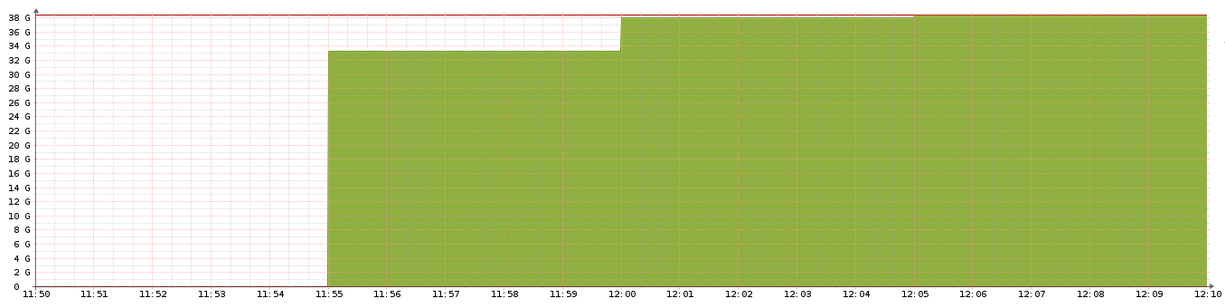
\includegraphics[scale=0.35]{images/pktgen_link_usage.png}
  \caption{Pktgen link usage (generated bandwidth at time x, graph displays an average of used bandwidth over 5 minutes}
  \label{fig:pktgenlink}
\end{figure}

\begin{figure}
  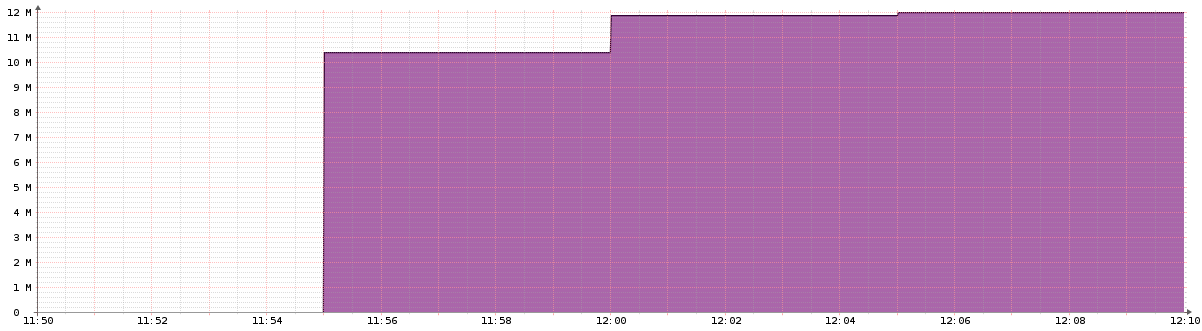
\includegraphics[scale=0.35]{images/pktgen_pps.png}
  \caption{Pktgen packets per second (generated packets per second at time x, graph displays the average transported pps over 5 minutes}
  \label{fig:pktgenpps}
\end{figure}

\newpage

\subsection{WARP}
A WARP client needs a server to respond to SYN packets, otherwise sessions are not opened up and there will be no traffic flowing. 
WARP has to be tested against a WARP server or against an application server. 
Thus in a setup as the one used for the other tests, servers A and B both needed to run WARP, one as a server and one as a client generating requests. RAW TCP communication is chosen for a first test. 
Sending a request of 64 bytes and responding with 64 bytes did not generate the maximum amount of pps expected, setting up the session using a three way handshake and transferring the data takes more CPU cycles, WARP seems to be limited regarding to the amount of packets per second it can send. WARP is capable of testing throughput up to the application level which makes it interesting for application layer testing.
To execute a benchmark for WARP, server B was connected to the network using two 40Gb/s interfaces. 
The benchmark increases the request and response sizes for every test. 4 million sessions are opened per test. The time it took to open the sessions, transfer the data and then close all 4 million sessions was registered. Tests were ran 3 times and the average value was written to a csv file. 
The results of this test for raw TCP traffic is shown in figures \ref{fig:rawtcplink} and \ref{fig:rawtcpsession}. 
WARP is also capable of testing HTTP session setup. The results of the benchmark for HTTP is visible in figures \ref{fig:httplink} and \ref{fig:httpsession}.
These figures show the packet sizes from the request and response along with the amount of sessions or the link usage.

\begin{figure}[H]
  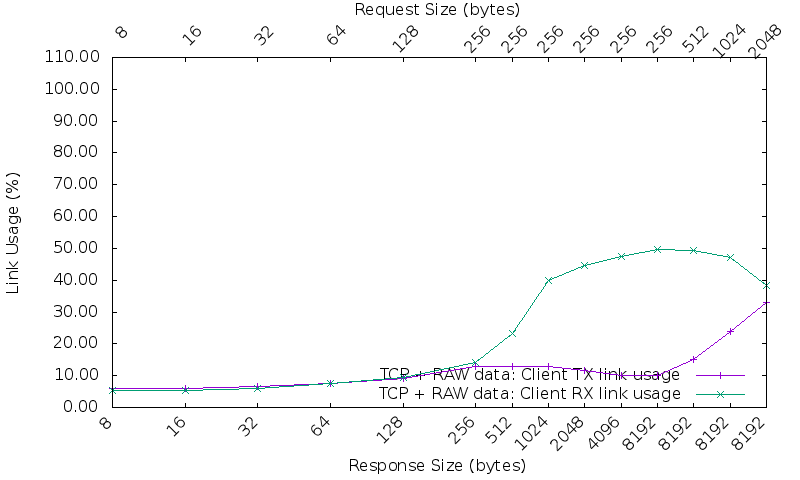
\includegraphics[scale=0.6]{images/raw_link_usage.png}
  \caption{Link usage for raw tcp (percentage of link usage versus the request(Rx) and response(Tx) size)}
  \label{fig:rawtcplink}
\end{figure}

\begin{figure}[H]
  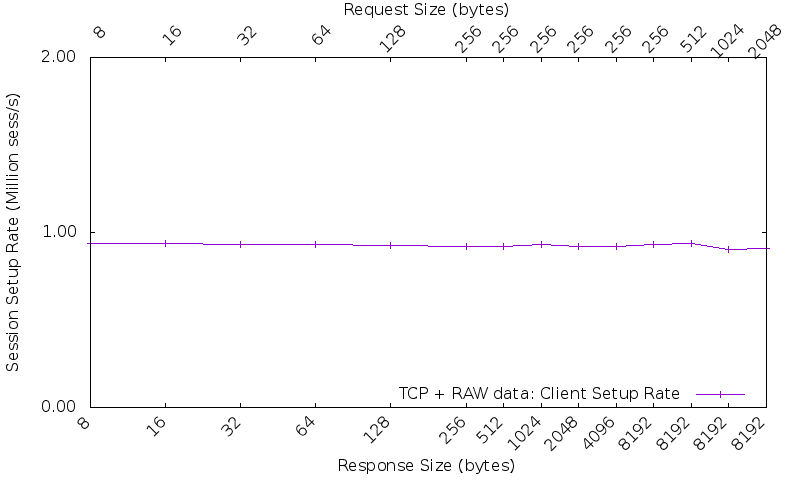
\includegraphics[scale=0.6]{images/raw_setup.png}
  \caption{Amount of session per second for raw tcp (amount of sessions (2-way) versus the request(Rx) and respond(Tx) size)}
  \label{fig:rawtcpsession}
\end{figure}

\begin{figure}[H]
  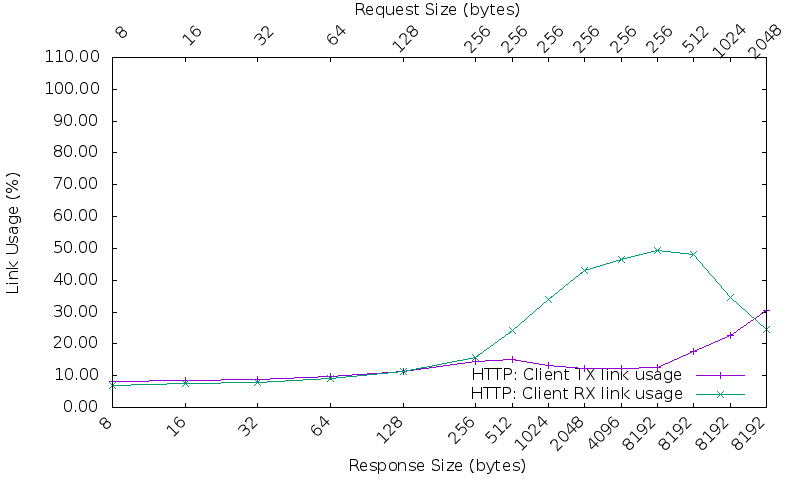
\includegraphics[scale=0.6]{images/http_link_usage.png}
  \caption{link usage for HTTP  (percentage of link usage versus the request(Rx) and response(Tx) size)}
  \label{fig:httplink}
\end{figure}

\begin{figure}[H]
  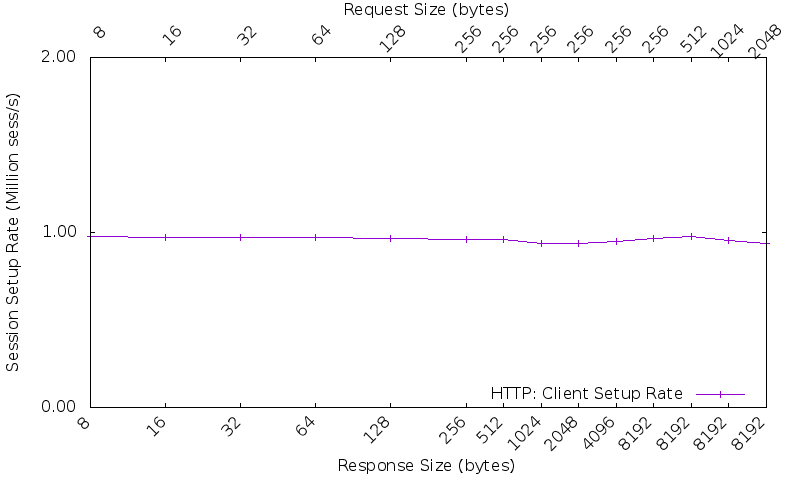
\includegraphics[scale=0.6]{images/http_setup.png}
  \caption{Amount of sessions per second for HTTP (amount of sessions (2-way) versus the request(Rx) and respond(Tx) size)}
  \label{fig:httpsession}
\end{figure}


\subsection{MoonGen}
MoonGen offers benchmark scripts to determine the machines capabilities. A single machine is connected to the switch using two 40Gb/s ports. Sending UDP traffic with a size of 1500 bytes resulted in a maximum of 24 Gb/s. When the smallest possible packets of 64 bytes are send over the line a maximum of 15Mpps is reached. When TCP is used on the same machine connected to the switch using two interfaces, a maximum of 10Gb/s was reached. These low values did not make MoonGen interesting enough since Pktgen is capable of reaching hardware limits. Figure \ref{fig:moongenlink} displays the maximum bandwidth reached while running different tests to get the maximum performance. 

\begin{figure}[H]
  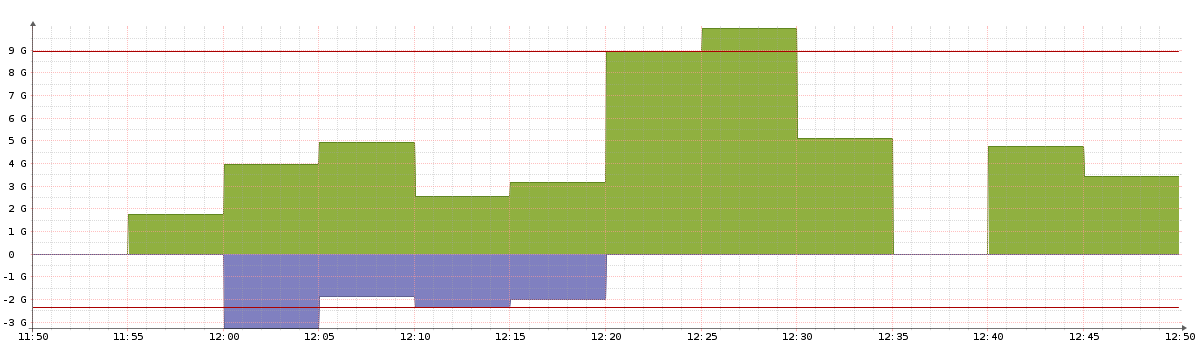
\includegraphics[scale=0.35]{images/moongen_link_usage.png}
  \caption{MoonGen link usage (changing packet sizes trying to find the limitations of MoonGen)}
  \label{fig:moongenlink}
\end{figure}





\chapter{Methodology}\label{ch:method}

In order to create a framework to get the limitations of the hardware and connecting infrastructure up to layer 7, use cases are formulated.
Only when the use cases are clear and there is an insight in the expected outcome, the correct applications can be selected for the framework.
The expected outcome is derived from the experiments. 

\section{Use cases}\label{sec:usecase}

Table \ref{tab:usecases} displays four different use cases. All serving a different purpose.
Use case 1 is designed to get the hardware limits of the NIC inside a host. Use case 2 is to get the limits of the  switching and routing hardware of the DUT.
Use case 3 will get the client and server limits up to layer 4. To handle TCP sessions, resources need to be allocated at client and server. 
Use case 4 is designed to get the limits of an application running on top of a kernel.  
Use cases 1 and 2 will show local limitations. 
When executing use cases 3 and 4 from a client to a server over a corporate network, using a statefull firewall, load balancers, aggregated links and active-standby machines.They will show the weakest link in the infrastructure towards the server.  
It should be noted that monitoring is in important part for showing the weakest link. 

\begin{table}[]
\centering
\caption{Use cases}
\label{tab:usecases}
\begin{tabular}{|l|l|l|l|}
\hline
NR & Use case                        & DUT            & Goal                                                                                             \\ \hline
UC1  & \begin{tabular}[c]{@{}l@{}}Bandwidth \\ generation\end{tabular}       & Client         & \begin{tabular}[c]{@{}l@{}}The goal is to see if the client is capable \\ of filling up the link and to reach the \\ maximum amount of pps \end{tabular} \\ \hline
UC2  & Throughput                    & Switch/router  & \begin{tabular}[c]{@{}l@{}}Generate the maximum amount of data in 2 ways \\ to make sure the hardware is able to forward\\ at line rate\end{tabular} \\ \hline
UC3  & TCP based                     & Client/Server  & Get the hardware limitations of the systems  \\ \hline
UC4  & Application             & \begin{tabular}[c]{@{}l@{}}Server and \\intermediate devices\end{tabular}         & \begin{tabular}[c]{@{}l@{}}The clients will overload the server with \\ requests at application level\end{tabular}  \\ \hline
\end{tabular}
\end{table}

\subsection{UC1}
In paragraph \ref{par:pps} it is stated that a 40Gb/s card needs to be able to handle 58 million packets with a size of 88 byte to handle a unidirectional stream of 40Gb/s.
Using PKTGEN, a tool on top of DPDK, TCP packets with a minimum size of 64 bytes (without inter frame gap, preamble and VLAN tag) can be created. This should generate 58 Mpps. To reach the 40Gb/s, larger packets have to be created. When the packet size is set to 1500 bytes, there have to be 3.3 Mpps to fill up the link. When Jumbo frames are used only 555 thousand packets per second are needed to fill up the link. When using PKTGEN on top of DPDK numbers like these can be reached using TCP traffic. When DPDK is used, the kernel cannot communicate to the devices anymore. So traffic statics cannot be read from the kernel. Monitoring on the switch ports connecting the servers is needed. 

\subsection{UC2}
The backplane of a switch should be able to forward traffic from one port to another at line speed. This should also be possible when the traffic is routed from one VLAN to the other. Routers should be able to rewrite packets at line rate. To test this a client and a server need to be connected to two different ports of the switch in a different segment or VLAN a high load should be generated from the client to the server, preferably the maximum link speed. Monitoring the ports of the switch using SNMP should show the same input rate on port 1 compared to the output rate of port 2.    

\subsection{UC3}
To get the limitations of the servers hardware when TCP is used, the kernel has to be bypassed. Using DPDK and WARP17 will show the limits of the hardware under load. As seen in the experiments in chapter \ref{ch:experiments}. The benchmark that was ran on a single machine running as client and server show the ability to open 1 million session per second, generating a maximum of 20Gb/s of RAW TCP traffic. Two tests need to be executed. A RAW TCP test between two different machines, and a test between client and server using HTTP. WARP17 is capable of talking HTTP, a layer 7 protocol. This should be the second test. Monitoring of the amount of successful and failed session has to be done on the client and server. When the API is used, detailed results can be retrieved as shown during the experimentation phase.   

\subsection{UC4}
WARP17 is capable of talking HTTP. This use case requires a web server running on one of the machines (the DTN). The client will use WARP17 to generate HTTP GET requests towards the DTN. The web server has to provide some files of different sizes. Warp can send a request for a certain file with a specified request size. Resources of the server and statefull devices on the path towards the server will be claimed opening up the sessions, By sending a million requests per second the machines will be experiencing a Denial of Service (DOS) like attack.


\section{Real world scenario}
The use cases mentioned in section \ref{sec:usecase} have to be tested in a real world scenario to see if they are useful. Therefore the infrastructure of a company was used to test this method.
Figure, \ref{fig:nikhefuva} shows the simplified infrastructure for the test between client and server. All tests performed, generated traffic for 90 seconds with a gap of 30 seconds before the next tests started in the same category. According to RFC2544 \cite{rfc2544} throughput tests need to take at least 60 seconds. The clients always initiated the sessions to the DTN.

\begin{figure}
  \includegraphics[scale=0.6]{images/nikhefuva.pdf}
  \caption{Infrastructure of real world scenario.}
  \label{fig:nikhefuva}
\end{figure}

\subsection{UC1}
Using PKTGEN on top of DPDK with a packet size of 64bytes generated a maximum of 42 Mpps towards the server. PKTGEN only sends from one source to one destination, also using just one source and destination port. The link from the switch to the router at the client side is an aggregated link build up from 4x 10Gb/s interfaces. Hashing algorithms decide what interface is used per stream. Since the combination is always the same and a switch's default hashing algorithm uses layer 2 addresses as input. The packets followed the same path, what ended up in a single 10Gb/s link towards the destination. The packet size needs to be increased after 2 minutes to 400bytes. This is the sweet spot for the amount of packets and bits traveling over the line towards the destination with the potential of sending 11Mpps and 39Gb/s of traffic to the server.  

\subsection{UC2}
Due to the hashing settings that cannot be changed without effect on the total environment, use case 2 does not need to be performed. A total of 40Gb/s cannot be reached.

\subsection{UC3}
Sending RAW TCP sessions between 2 servers using WARP17 with different packet sizes should provide a good representation of the capabilities of the servers and the intermediate devices in the path from source to destination. 
The server should be running WARP17, acting as a TCP RAW server listening on 100 ports. Sending responses of a specified size when requests come in. The client could be configured to use 40 thousand ports for the requests, targeting the 100 ports at the servers side. This makes a total of 4 million possible flows between client and server. Request and response sizes can be the same at every run. The request/response sizes depend on the link speed, in this case proper values are, 64, 256, 512, 1024 and 2048 bytes. 

\subsection{UC4}
A web server needs to be setup offering a couple of files from a RAMdisk, this should be done to make sure disk IO will not become the bottleneck for the tests. Using WARP17 at the client side requesting the files from the DTN. NGINX was capable of delivering 11Gb/s inside the experimentation environment. This test will get the limits of the infrastructure towards the DTN or from the DTN itself running the application. 

\

%What will be tested?

%Describe the test environment and the upcoming tests
%Why are these test useful? 
%What results are we looking for?
%What are the values/specific settings for these tests?
%What will be monitored on the receiver or sender side.
%Why am I monitoring this.
%What conclusion would I like to draw out of the test results.
 

%TEST environment. 
%2 identical machines running different operating systems at first.
%After preliminary tests the OS might be changed to one OS for final tests.
%In the middle sits a Juniper QFX10k2 as a router/switch.

%Limitations known inside the PCI buss connecting the card. Limited to 40 million packets per second.




%Ubuntu:
%./pktgen_sample03_burst_single_flow.sh -i eth2 -m 3c:8a:b0:34:2f:f0 -d 10.10.10.10 -s 9000
%-i = interface
%-m = destination mac
%-d = destination address
%-s = size
%-t = threads

%FreeBSD:
%./pkt-gen -i ixl0 -f tx -d 10.10.10.20 -s 10.10.10.10 -S 68:05:ca:32:17:e0 -l 9000
%-i = interface
%-f = function
%-d = destination ip addres
%-s = source ip address
%-S = source mac address
%-l = length
%-R = Rate (amount of packets per second)




\chapter{Results}\label{ch:results}

From the experiments described in chapter \ref{ch:experiments} a framework was created and tested in chapter \ref{ch:method}. 
The 'easy to use' tools like iPerf3, hping and BoNeSi are useful for quick tests. But when it comes to representative session based application testing these tools do not offer the solution for high speed networks. 
As these 'easy to use' tools all require the kernel to talk to the hardware. As described in section \ref{sub:dpdk}, DPDK is able to bypass the kernel and talk to the interface directly. Cores and memory needs to be dedicated to generate traffic.  

\section{Infrastructure}
The network at 'company x' as it is shown in figure \ref{fig:testenv} is a simplified representation.
The detailed infrastructure used during the real world test is displayed in figure \ref{fig:companyx} 
Since all the network hardware is redundant and a single device failures cannot result in a total downtime the figure and therefore the monitoring gets more complicated.
The server is connected to a data center layer that is spread over two physical locations, one serving as the active and the other as the passive environment.
To minimize the unnecessary traffic between the data centers an overlay technique is used. This overlay also blocks broadcast storms at one location spreading to the other location.  
When traffic does not arrive at the destination, detailed measurements are needed at every device for every link to determine where the traffic gets dropped.   

\begin{figure}[H] 
  \includegraphics[scale=0.4]{images/companyx.pdf}
  \caption{Detailed visualization of real world scenario.}
  \label{fig:companyx}
\end{figure}

\section{Data Plane Development Kit based tools}
Since none of the use cases require the 'easy to use' tools, simply due to the fact that these tools do not reach the performance required for this research. 
The results of the DPDK based applications are explained during the use case performance tests on the real world scenario.
  
\subsection{pktgen}
Pktgen was used to get the limitations from the test hardware: It was already known that the maximum amount of pps is a hardware limitation inside the PCI Express Bus. 
The maximum link speed can be reached when packets of 400 bytes are used. To get an idea of the throughput over the entire path from client to server, pktgen is used to setup a UDP stream from the client to the server. 
The source IP address and port towards the destination IP address and port are the same. Since aggregated interfaces are used from the test switch to the router, the hashing algorithm in the switch limits the traffic to only one link filled up by this test. 
Figure \ref{fig:surftest} shows a maximum throughput of 7 Gb/s at 20:40. This was transported to company x and delivered to router1, the logical aggregation of the physical routers 1a and 1b. From here it is important to know what lines are used to transport the traffic towards the firewall.
Figures \ref{fig:testrealusageae112} and \ref{fig:testrealusageae113} display the graphs of the traffic that went out of the aggregated interfaces connecting router1 to the firewall cluster and the links connecting the firewalls to the DCI switches inside the data center. The white gaps between send and received data, is traffic that got lost during the execution of the use cases. Data points above zero represent data that went from server to client and data points below zero represent data from client to server. 
   
\begin{figure}[H]
  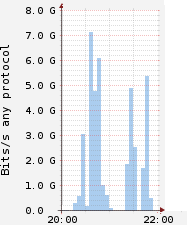
\includegraphics[scale=0.5]{images/test-link-usage.png}
  \caption{Bandwidth utilization of real world tests during the time window of the tests.}
  \label{fig:surftest}
\end{figure}

\begin{figure}[H]
  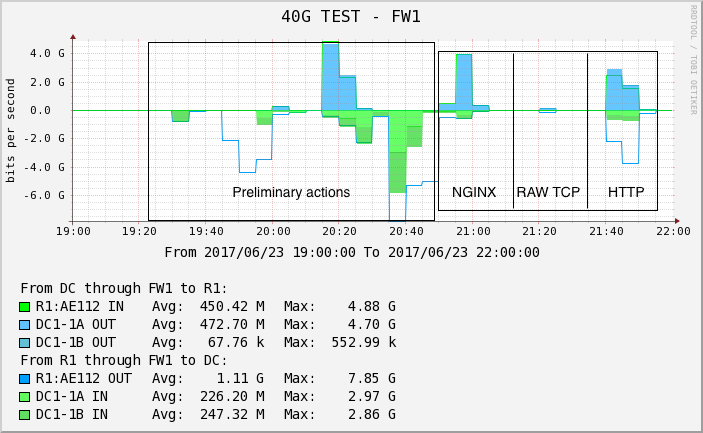
\includegraphics[scale=0.5]{images/real-ae112.png}
  \caption{Bandwidth utilization of links between router1, firewall1 and DC1 during the time window of the tests, spikes represent an executed test.}
  \label{fig:testrealusageae112}
\end{figure}

\begin{figure}[H]
  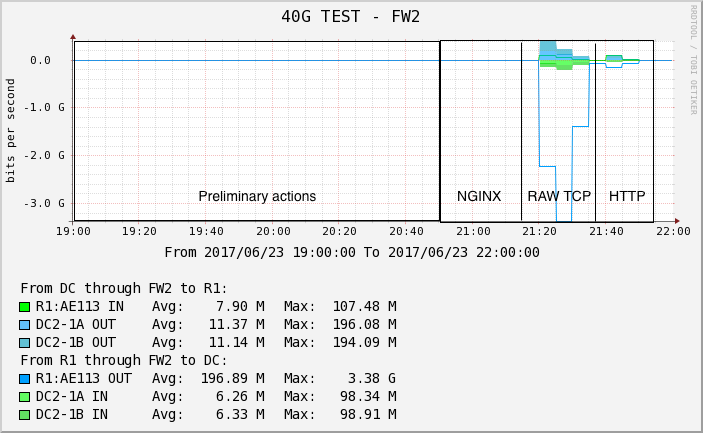
\includegraphics[scale=0.5]{images/real-ae113.png}
  \caption{Bandwidth utilization of links between router1, firewall2 and DC2 during the time window of the test, the spike represents the moment of a fail over to the secondary machine.}
  \label{fig:testrealusageae113}
\end{figure}



% 20:42 - 20:50 PKTGEN UDP en TCP
% 20:54 - 21:00 WARP - NGINX
% 21:21 - 21:30 WARP - RAW TCP
% 21:42 - 22:00 WARP - HTTP

\subsection{WARP}
From the benchmark results performed on WARP in chapter \ref{ch:experiments} it is known WARP is capable of generating almost a million sessions per second. 
WARP was used to run three tests. WARP needs to be commanded using its own syntax. The command file that was used for the NGINX server test and the WARP HTTP server test can be found in appendix \ref{appendix:software}. As WARP runs on top of DPDK, the DPDK commands point to resources that will be claimed by DPDK. As an example:

\begin{verbatim}
./build/warp17 -c ff -n 4 -m 32768 -- --qmap-default max-c \
--ucb-pool-sz 32768 --tcb-pool-sz 32768 --cmd-file \
test-client-nginx-http.txt 
\end{verbatim} 

Figure \ref{fig:warptime} shows the results of the three experiments. 
Therefore, WARP was used to retrieve a 500 Kbyte file from an NGINX web server running on server A.
The file was placed on a RAM disk to make sure disk IO would not be the bottleneck during the performance tests. 
This test is executed starting at 20:50 and it ran until 21:00. The request size is increased every 90 seconds with an interval of 30 seconds between the tests.
During this test the following request sizes where used: 64, 256, 512, 1024 and 2048 bytes. 
Figure \ref{fig:realnginx} shows that the amount of traffic leaving the server goes above 4Gb while only 0.6 Gb of requests are coming in on the receiving end. 
This matches the values shown in figure \ref{fig:testrealusageae112}. \\
Rate limiting at the NGINX server on the receiving end (allowing the server to accept a maximum of 40 thousand concurrent sessions) made sure nothing broke. The services got depleted at the machine, this made the service unavailable for other users.
The graphs show us that traffic was not lost during this test.

\begin{figure}[]
  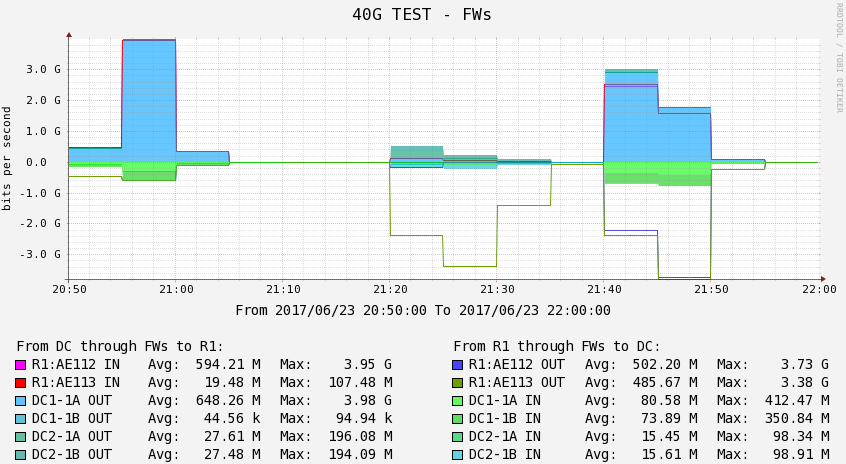
\includegraphics[scale=0.5]{images/warp-timeline.png}
  \caption{Time line of the preformed tests using WARP displaying the bandwidth usage over time}
  \label{fig:warptime}
\end{figure}

\begin{figure}
  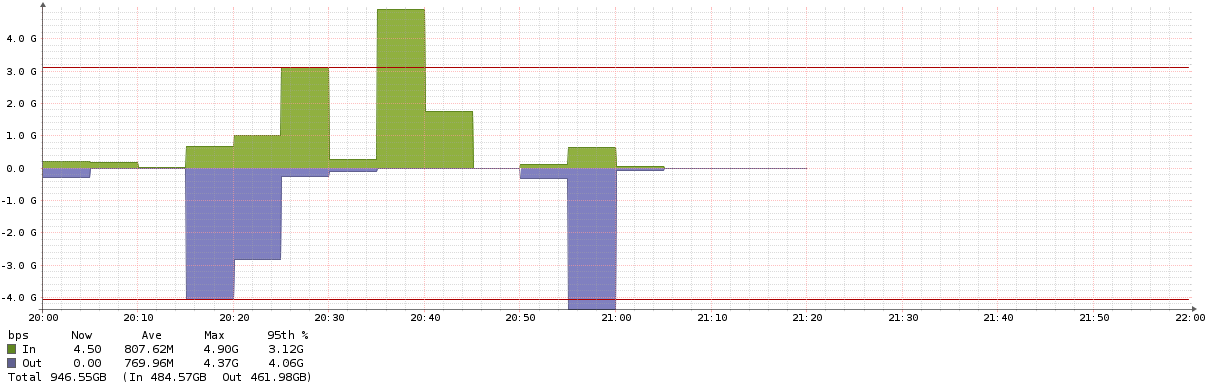
\includegraphics[scale=0.35]{images/real-nginx.png}
  \caption{Bandwidth utilization server A during NGINX test, measurements from servers perspective }
  \label{fig:realnginx}
\end{figure}


At 21:20 the next test was started, generating a maximum amount of RAW TCP sessions (this test is performed on OSI layer 4 by sending TCP RAW request and responses) from client to server both running WARP and using 32GB of memory and all cores to generate traffic.
Request and response sizes chosen for this tests are: 64, 256, 512, 1024 and 2048 bytes. 
Since WARP needs control of the interfaces, the server's kernel will not display any traffic on the interfaces. 
The measurements all came from the uplink and downlink interfaces of the devices in the path as shown in figure \ref{fig:companyx} represented by "AE112" and "AE113"
Sessions statistics where not registered due to logging problems in the firewall environment. 
Chapter \ref{ch:experiments} shows that the benchmark value of 1 million sessions per second is generated, no differences are observed at different packets sizes. 
Only 10\% of the link is utilized at the starting point of the benchmark test as displayed in \ref{fig:rawtcplink}. 
The graph in figure \ref{fig:testrealusageae112} doesn't display any traffic at 21:20. This is the moment the RAW TCP test was started while figure \ref{fig:surftest} displays traffic towards the tested network. 
The graph in figure \ref{fig:testrealusageae113} displays the load. When the test started, the active firewall crashed and a failover to the passive machine is the result. Log messages retrieved from connected routers also display BGP session failures from the formerly-active firewall. 
This graph also displays the difference between traffic send from the router to the firewall and the traffic received by the downstream switch. 
Input is 3Gb and output is in the range of 200 - 300 Mb. The firewall had a rule accepting all the traffic from the source range of the test machines.
The firewalls are not capable of handling this amount of sessions per second. Due to time limitations this test could not be performed again to figure out the limitations.  
When the test was finished, the firewalls started to recover. \\ 

The firewall environment was restored to the way it was in the beginning of the first test.
At 21:40 the last test is started between server and client, again both running WARP. Generating the maximum amount of HTTP sessions using 32GB of memory and all available cores.
Generating a GET request and responding with a 200-(OK) message from the server running WARP instead of NGINX.  
From the experimental phase of this research it is known that WARP is capable of handling more request per second than NGINX can. This last test is executed to find the limits of intermediate hardware when HTTP sessions are opened up in a fast rate.
Message sizes for the tests are : 64, 256, 512, 1024 and 2048 bytes. Request and response size are equal. 
With the information from the benchmark in chapter \ref{ch:experiments} the limitations of client and server are known. 
From the tests at 21:20 it is known the firewalls will die when to many sessions per second come in. The same behavior is expected during this test.
Figure \ref{fig:testrealusageae112} shows 4Gb/s going into the firewall and only 500Mb/s of HTTP traffic arriving at the other side.
This means that the firewall was not able to handle the amount of sessions per second and the machines stop functioning. 
Management sessions broke down and traffic got lost.



\chapter{Conclusion}\label{ch:conclusion}
From the tool assessment performed in chapter \ref{ch:experiments} and the tests described in chapter \ref{ch:method}, results are gathered and described in chapter \ref{ch:results}.
The results, executed according to current standards and best practices, allow to draw conclusions on tool suitability and the necessary characteristics of high-bandwidth session based throughput tests in a real-world environment. \\
When it comes to generating session based high bandwidth throughput testing, DPDK should be used in combination with pktgen in order to reach hardware limitations. 
Using DPDK in combination with WARP creates the possibility to generate traffic at the application layer. 
The kernel based tools could not provide the results this research was looking for. 

During this research, the limitations of the hardware used in the experimental setup were found by executing the tests. 
The tests can be used as a guideline to find the hardware limits in the path from client to server. 
T1 revealed  a limitation for the amount of packets per second in the PCI Express bus. 
T2 was used to get the maximum possible throughput from client to server, the hashing settings were shown to be a limitation in the setup as expected.
T3 revealed the hardware limits for client and server with regards to the amount of sessions and bandwidth usage.
Next to the hardware  limits T3 revealed a limitation of a stateful firewall in the path towards the destination, the overload behavior of the firewall is also known by executing this test.\\ 
T4 stressed an application to get the performance limits for this specific application.
 
These tests should be used to get a better insight in the limitations of an infrastructure that is used to provide services.
Combining DPDK with pktgen and WARP can reveal the limits of an infrastructure.
To perform high bandwidth session based throughput tests up to layer 3, pktgen on top of DPDK is capable of reaching hardware limits.
For application layer link testing, WARP is the framework to use. Support for other applications must be added to WARP in order to improve the employability, but the start looks promising.
The use of different kernels did not show any major differences in the results of executed kernel based application tests during this research. 

The exact limit of the firewall was not found, it is only known that one server using WARP can generate the amount of sessions per second to make the system fail.
By increasing the amount of sessions step by step we could have pinpointed the amount of sessions where the firewall started failing.

%When looking at the results of the real world test one could argue if it is useful to equip a web server with a 40Gb/s interface when the maximum HTTP performance using WARP is below 20Gb/s.
%When running NGINX as a web server, a 40Gb/s NIC is not economically viable for the hardware used during this research. 

\section{Suitability of the Data Plane Development Kit}
The Data Plane Development Kit is still a work in progress, and today we see only the beginning of its potential being harnessed for network load testing. New tools that use the power of DPDK are introduced every year:
Pktgen (2013), MoonGen(2014), T-rex (2015), WARP(2016).
The possibilities to test up to layer 7 in the OSI model are now becoming available to system and network administrators. 
Current tooling is capable of generating a million sessions per second using simple server hardware. 
DPDK applications supporting IPv6 and multiple application layer protocols are needed to improve infrastructures in order to offer services. 

\section{Future Work}
The hashing algorithm used at Nikhef's core network limited the performance tests to 10Gb/s. Using 4 clients or changing the hashing settings should result in more bandwidth utilization. 
By doing this, the other limitation this research was looking for such as the amount of packets per second being a bottleneck can be reached. Further analysis on the Data Center Infrastructure layer at company x can be performed. 
%A close collaboration with the engineers of company x should help them to overcome the problems before the network goes into production. 

During this project an attempt was  made to use an IBM Power8 machine (server E) to generate traffic at 100Gb/s. Because of problems during compilation and memory allocation this attempt had to be abandoned due to time constraints.

This project used HTTP version 1.1 for application testing. Support for more protocols need to be added to WARP to make it more powerful. 
Currently WARP supports IPv4 only. When IPv6 is supported, the performance should be tested using IPv6. 
Monitoring in WARP should be improved, currently the API provides the only way of getting detailed results.
NGINX was made available for DPDK recently. Running WARP towards a DPDK NGINX server should provide the capabilities of NGINX when it does not rely on kernel interrupts. \\

DPDK supports multiple NICs. During the project an effort was made to start generating traffic over 100Gb/s Mellanox cards.
This was successful up to 60Gb/s TCP traffic, until the system crashed for reasons that could not be determined within the scope of this project. 
The proposed tests in this research paper need to be run using the Mellanox cards. 
Support and limitations for different 100Gb/s cards need to be researched.

The Generation 3, 8 lane PCI express cards are a limiting factor as shown in this paper. 
Further investigations could look into the limitations of 16-lane PCIe and its associated scaling behavior.

Intel offers a guide to improve the throughput for the XL710 40Gb/s card for the Linux kernel \cite{intellinuxguidxl710}. 
This guideline provides kernel settings that might improve the results for the kernel based tools.
During this research the guideline was not used to improve the kernel settings, the reason for this is that the settings are dependent on the application that is ran on top of the kernel. 
This research, due to time constraints focused on the DPDK tooling. Tweaking the kernel for all the tools in table \ref{table:tools} is out of scope for this research while it would be very interesting to know if the proposed settings from the guide will impact the performance of the kernel based tools. 


% UNCOMMENT THIS TO PRINT ONLY CITED REFERENCES
\nocite{*}
\bibliographystyle{plainnat}
\bibliography{report}
\begin{appendices}
\appendix
\thispagestyle{empty}

\chapter{}\label{appendix:acronym}

\begin{table}[H]
\centering
\caption{Used Acronyms}
\label{table:acronyms}
\begin{tabular}{l|l}
\hline
\textbf{Acronym}                  & \textbf{Definition}  \\ \hline
DTN & Data Transfer Node \\ \hline
CLI & Command Line Interface \\ \hline
PPS & packets per second \\ \hline
Gb/s & Gigabit per second \\ \hline
DPDK & Data Plane Development Kit \\ \hline
ISP & Internet service provider \\ \hline
QSFP & Quad Small Form-factor Pluggable \\ \hline
DOS & Denial Of Service \\ \hline
DDOS & Distributed Denial Of Service \\ \hline
FCS & Frame check sequence \\ \hline
MTU & Maximum Transmission Unit \\ \hline
OSI & Open System Interconnection \\ \hline
NIC & Network Interface Card \\ \hline
TCP & Transport Control Protocol \\ \hline
UDP & User Datagram Protocol \\ \hline
ICMP & Internet Control Message Protocol \\ \hline
OS & Operating System \\ \hline
LAN & Local Area Network \\ \hline
VLAN & Virtual LAN \\ \hline
IP & Internet Protocol \\ \hline
HTTP & Hyper Text Transport Protocol \\ \hline
MTU & Maximum Transmission Unit \\ \hline
SNMP & Simple Network management Protocol \\ \hline
RFC & Request For Comment \\ \hline
DUT & Device Under Tests \\ \hline
CPU & Central Processing Unit \\ \hline
UC & Use Case \\ \hline
API & Application Programmable Interface \\ \hline
EVPN & Ethernet Virtual Private Network \\ \hline
DWDM & Dense Wave Division Multiplexing \\ \hline
\end{tabular}
\end{table}


\thispagestyle{empty}

\chapter{}\label{appendix:software}
\section{Software}

\textbf{Software used during research:}
\begin{itemize}
\item{Ubuntu 16.04 LTS}
\item{FreeBSD 11.0}
\item{DPDK 16.11}
\item{pktgen(dpdk) 3.3.4}
\item{WARP 1.4}
\item{Moongen}
\item{iPerf 3.1.3}
\item{hping 3}
\item{Bonesi V0.3}
\end{itemize}

\begin{landscape}
\section{benchmark test}\label{app:benchmark}

\textbf{Benchmark script for WARP:}\\
This script is provided with the application source \cite{juniperwarp17bm}.
\begin{verbatim}
import sys
import time

from functools import partial

sys.path.append('../../python')
sys.path.append('../../api/generated/py')
sys.path.append('../../ut/lib')

from warp17_api import *

from b2b_setup import *

from warp17_common_pb2    import *
from warp17_l3_pb2        import *
from warp17_server_pb2    import *
from warp17_client_pb2    import *
from warp17_app_raw_pb2   import *
from warp17_app_http_pb2  import *
from warp17_test_case_pb2 import *
from warp17_service_pb2   import *

# 4M sessions
sip_cnt = 1
dip_cnt = 1
sport_cnt = 40000
dport_cnt = 100

sess_cnt = sip_cnt * dip_cnt * sport_cnt * dport_cnt
serv_cnt = dip_cnt * dport_cnt

expected_rate = 1000000
run_cnt = 3

def die(msg):
    sys.stderr.write(msg + ' Should cleanup but we just exit..\n')
    sys.exit(1)

def get_server_test_case(protocol, app, req_size, resp_size):
    l4_scfg = L4Server(l4s_proto=protocol,
                       l4s_tcp_udp=TcpUdpServer(tus_ports=b2b_ports(dport_cnt)))
    app_scfg = {
        RAW: AppServer(as_app_proto=RAW,
                       as_raw=RawServer(rs_req_plen=req_size,
                                        rs_resp_plen=resp_size)),
        HTTP: AppServer(as_app_proto=HTTP,
                        as_http=HttpServer(hs_resp_code=OK_200,
                                           hs_resp_size=resp_size))
    }.get(app)

    return TestCase(tc_type=SERVER, tc_eth_port=1, tc_id=0,
                    tc_server=Server(srv_ips=b2b_sips(1, sip_cnt),
                                     srv_l4=l4_scfg,
                                     srv_app=app_scfg),
                    tc_criteria=TestCriteria(tc_crit_type=SRV_UP,
                                             tc_srv_up=serv_cnt),
                    tc_async=False)

def get_client_test_case(protocol, app, req_size, resp_size):
    l4_ccfg = L4Client(l4c_proto=protocol,
                       l4c_tcp_udp=TcpUdpClient(tuc_sports=b2b_ports(sport_cnt),
                                                tuc_dports=b2b_ports(dport_cnt)))
    rate_ccfg = RateClient(rc_open_rate=Rate(),
                           rc_close_rate=Rate(),
                           rc_send_rate=Rate())

    delay_ccfg = DelayClient(dc_init_delay=Delay(d_value=0),
                             dc_uptime=Delay(),
                             dc_downtime=Delay())

    app_ccfg = {
        RAW: AppClient(ac_app_proto=RAW,
                       ac_raw=RawClient(rc_req_plen=req_size,
                                        rc_resp_plen=resp_size)),
        HTTP: AppClient(ac_app_proto=HTTP,
                        ac_http=HttpClient(hc_req_method=GET,
                                           hc_req_object_name='/index.html',
                                           hc_req_host_name='www.foobar.net',
                                           hc_req_size=req_size))
    }.get(app)

    return TestCase(tc_type=CLIENT, tc_eth_port=0,
                    tc_id=0,
                    tc_client=Client(cl_src_ips=b2b_sips(0, sip_cnt),
                                     cl_dst_ips=b2b_dips(0, dip_cnt),
                                     cl_l4=l4_ccfg,
                                     cl_rates=rate_ccfg,
                                     cl_delays=delay_ccfg,
                                     cl_app=app_ccfg),
                    tc_criteria=TestCriteria(tc_crit_type=CL_ESTAB,
                                             tc_cl_estab=sess_cnt),
                    tc_async=False)

def configure_server_port(warp17_call, protocol, app, req_size, resp_size):
    pcfg = b2b_port_add(eth_port=1, def_gw=Ip(ip_version=IPV4, ip_v4=0))
    b2b_port_add_intfs(pcfg,
                       [
                        (Ip(ip_version=IPV4, ip_v4=b2b_ipv4(eth_port=1, intf_idx=i)),
                         Ip(ip_version=IPV4, ip_v4=b2b_mask(eth_port=1, intf_idx=i)),
                         b2b_count(eth_port=1, intf_idx=i)) for i in range(0, dip_cnt)
                       ])

    if warp17_call('ConfigurePort', pcfg).e_code != 0:
        die('Error configuring port 1!')

    scfg = get_server_test_case(protocol, app, req_size, resp_size)
    if warp17_call('ConfigureTestCase', scfg).e_code != 0:
        die('Error configuring server test case')

def configure_client_port(warp17_call, protocol, app, req_size, resp_size):
    pcfg = b2b_port_add(eth_port=0, def_gw=Ip(ip_version=IPV4, ip_v4=0))
    b2b_port_add_intfs(pcfg,
                       [
                        (Ip(ip_version=IPV4, ip_v4=b2b_ipv4(eth_port=0, intf_idx=i)),
                         Ip(ip_version=IPV4, ip_v4=b2b_mask(eth_port=0, intf_idx=i)),
                         b2b_count(eth_port=0, intf_idx=i)) for i in range(0, sip_cnt)
                       ])

    if warp17_call('ConfigurePort', pcfg).e_code != 0:
        die('Error configuring port 0!')

    ccfg = get_client_test_case(protocol, app, req_size, resp_size)
    if warp17_call('ConfigureTestCase', ccfg).e_code != 0:
        die('Error configuring client test case')


def run_test(protocol, app, req_size, resp_size):
    env = Warp17Env(path='./test_2_perf_benchmark.ini')
    warp17_pid = warp17_start(env=env, exec_file='../../build/warp17',
                              output_args=Warp17OutputArgs(out_file='/tmp/test_2_perf.out'))
    warp17_wait(env=env, logger=LogHelper(name='benchmark',
                                          filename='/tmp/test_2_perf.log'))

    warp17_call = partial(warp17_method_call, env.get_host_name(),
                          env.get_rpc_port(), Warp17_Stub)

    configure_server_port(warp17_call, protocol, app, req_size, resp_size)
    configure_client_port(warp17_call, protocol, app, req_size, resp_size)
    timeout_s = int(sess_cnt / float(expected_rate)) + 2

    if warp17_call('PortStart', PortArg(pa_eth_port=1)).e_code != 0:
        die('Error starting server test cases!')

    if warp17_call('PortStart', PortArg(pa_eth_port=0)).e_code != 0:
        die('Error starting client test cases!')

    time.sleep(timeout_s)

    result = warp17_call('GetTestStatus', TestCaseArg(tca_eth_port=0,
                                                      tca_test_case_id=0))
    if result.tsr_state != PASSED:
        die('Test case didn\'t pass: ' + str(result))

    start_time = result.tsr_stats.tcs_start_time
    end_time = result.tsr_stats.tcs_end_time

    # start and stop ts are in usecs
    duration = (end_time - start_time) / float(1000000)
    rate = sess_cnt / duration
    txr = result.tsr_link_stats.ls_tx_pkts / duration
    rxr = result.tsr_link_stats.ls_rx_pkts / duration
    link_speed_bytes = float(result.tsr_link_stats.ls_link_speed) * 1024 * 1024 / 8
    tx_usage = min(float(result.tsr_link_stats.ls_tx_bytes) * 100 / duration / link_speed_bytes, 100.0)
    rx_usage = min(float(result.tsr_link_stats.ls_rx_bytes) * 100 / duration / link_speed_bytes, 100.0)

    warp17_stop(env, warp17_pid, force=True)
    return (rate, txr, rxr, tx_usage, rx_usage)

def run_test_averaged(descr, protocol, app, req_size, resp_size, run_cnt):
    results = [run_test(protocol, app, req_size, resp_size)
               for i in range(0, run_cnt)]
    avgs = [sum(result, 0.0) / run_cnt for result in zip(*results)]

    # Print as csv
    print '%(descr)s,%(req_size)u,%(resp_size)u,%(rate).0f,%(txr).0f,%(rxr).0f,%(txu).2f,%(rxu).2f' % \
           {
            'descr': descr, 'req_size': req_size, 'resp_size': resp_size,
            'rate': avgs[0], 'txr': avgs[1], 'rxr': avgs[2],
            'txu': avgs[3], 'rxu': avgs[4]
           }

def run():

    # Print csv header
    print 'Description, req_size, resp_size, rate, tx pps, rx pps, tx usage, rx usage'

    # TCP RAW
    tcp_raw_cfg = [(8, 8), (16, 16), (32, 32), (64, 64), (128, 128),
                   (256, 256), (256, 512), (256, 1024), (256, 2048), (256, 4096),
                   (256, 8192), (512, 8192), (1024, 8192), (2048, 8192)]

    for (req_size, resp_size) in tcp_raw_cfg:
        run_test_averaged('TCP request={req!s}b response={resp!s}b'.format(req=req_size,
                                                                           resp=resp_size),
                          TCP, RAW, req_size, resp_size, run_cnt)

    # HTTP
    http_cfg = [(8, 8), (16, 16), (32, 32), (64, 64), (128, 128),
                (256, 256), (256, 512), (256, 1024), (256, 2048), (256, 4096),
                (256, 8192), (512, 8192), (1024, 8192), (2048, 8192)]

    for (req_size, resp_size) in http_cfg:
        run_test_averaged('HTTP request={req!s}b response={resp!s}b'.format(req=req_size,
                                                                            resp=resp_size),
                          TCP, HTTP, req_size, resp_size, run_cnt)

if __name__ == '__main__':
    run()
\end{verbatim}

\textbf{Benchmark script for Moongen:}\\
This script is provided with the application source \cite{moongenbm}.
\begin{verbatim}
local mg                = require "moongen"
local memory    = require "memory"
local device    = require "device"
local stats             = require "stats"
local log               = require "log"

function configure(parser)
        parser:description("Generates TCP SYN flood from varying source IPs, supports both IPv4 and IPv6")
        parser:argument("dev", "Devices to transmit from."):args("*"):convert(tonumber)
        parser:option("-r --rate", "Transmit rate in Mbit/s."):default(10000):convert(tonumber)
        parser:option("-i --ip", "Source IP (IPv4 or IPv6)."):default("10.0.0.1")
        parser:option("-d --destination", "Destination IP (IPv4 or IPv6).")
        parser:option("-f --flows", "Number of different IPs to use."):default(100):convert(tonumber)
end

function master(args)
        for i, dev in ipairs(args.dev) do
                local dev = device.config{port = dev}
                dev:wait()
                dev:getTxQueue(0):setRate(args.rate)
                mg.startTask("loadSlave", dev:getTxQueue(0), args.ip, args.flows, args.destination)
        end
        mg.waitForTasks()
end

function loadSlave(queue, minA, numIPs, dest)
        --- parse and check ip addresses
        local minIP, ipv4 = parseIPAddress(minA)
        if minIP then
                log:info("Detected an %s address.", minIP and "IPv4" or "IPv6")
        else
                log:fatal("Invalid minIP: %s", minA)
        end

        -- min TCP packet size for IPv6 is 74 bytes (+ CRC)
        local packetLen = ipv4 and 60 or 74

        -- continue normally
        local mem = memory.createMemPool(function(buf)
                buf:getTcpPacket(ipv4):fill{
                        ethSrc = queue,
                        ethDst = "12:34:56:78:90",
                        ip4Dst = dest,
                        ip6Dst = dest,
                        tcpSyn = 1,
                        tcpSeqNumber = 1,
                        tcpWindow = 10,
                        pktLength = packetLen
                }
        end)

        local bufs = mem:bufArray(128)
        local counter = 0
        local c = 0

        local txStats = stats:newDevTxCounter(queue, "plain")
        while mg.running() do
                -- fill packets and set their size 
                bufs:alloc(packetLen)
                for i, buf in ipairs(bufs) do
                        local pkt = buf:getTcpPacket(ipv4)

                        --increment IP
                        if ipv4 then
                                pkt.ip4.src:set(minIP)
                                pkt.ip4.src:add(counter)
                        else
                                pkt.ip6.src:set(minIP)
                                pkt.ip6.src:add(counter)
                        end
                        counter = incAndWrap(counter, numIPs)

                        -- dump first 3 packets
                        if c < 3 then
                                buf:dump()
                                c = c + 1
                        end
                end
                --offload checksums to NIC
                bufs:offloadTcpChecksums(ipv4)

                queue:send(bufs)
                txStats:update()
        end
        txStats:finalize()
end

\end{verbatim}

\section{scripts used during the tests}\label{app:realworld}

\textbf{Script used during the real world pktgen test:}\\
It starts of sending 64 byte frames, where after 400 byte frames are send to the destination.

\begin{verbatim}
set ip src 0 1.2.3.4/24
set ip dst 0 4.3.2.1
set mac 0 ff:ff:ff:ff:ff:ff
proto tcp 0
set 0 size 64
sleep 30
start 0
sleep 90
stop 0
set 0 size 400
sleep 30
start 0
sleep 90
stop 0
\end{verbatim}

\textbf{Scripts to perform WARP tests during real world test:\\}
\textbf{Server responding to requests from client using WARP}:

\begin{verbatim}
#Set client IP on interface
add tests l3_intf port 0 ip 1.2.3.4 mask 255.255.255.0
add tests l3_gw port 0 gw 1.2.3.1 

add tests server tcp port 0 test-case-id 0 src 1.2.3.4 1.2.3.4 sport 80 180
set tests server http port 0 test-case-id 0 200-OK resp-size 64

add tests server tcp port 0 test-case-id 1 src 1.2.3.4 1.2.3.4 sport 80 180
set tests server http port 0 test-case-id 1 200-OK resp-size 256

add tests server tcp port 0 test-case-id 2 src 1.2.3.4 1.2.3.4 sport 80 180
set tests server http port 0 test-case-id 2 200-OK resp-size 512

add tests server tcp port 0 test-case-id 3 src 1.2.3.4 1.2.3.4 sport 80 180
set tests server http port 0 test-case-id 3 200-OK resp-size 1024

add tests server tcp port 0 test-case-id 4 src 1.2.3.4 1.2.3.4 sport 80 180
set tests server http port 0 test-case-id 4 200-OK resp-size 2048

start tests port 0
show tests ui
\end{verbatim}

\textbf{Client requesting a file from a server (can be run to an NGINX server or to a WARP server)}:
\begin{verbatim}
add tests l3_intf port 0 ip 4.3.2.1 mask 255.255.255.0
add tests l3_gw port 0 gw 4.3.2.254

add tests client tcp port 0 test-case-id 0 src 4.3.2.1 4.3.2.1 sport \ 
10000 50000 dest 1.2.3.4 1.2.3.4 dport 80 180
set tests client http port 0 test-case-id 0 GET "1.2.3.4" \
/files/500K.img req-size 64

set tests timeouts port 0 test-case-id 0 init 30
set tests timeouts port 0 test-case-id 0 uptime 1
set tests timeouts port 0 test-case-id 0 downtime 0
set tests criteria port 0 test-case-id 0 run-time 90

add tests client tcp port 0 test-case-id 0 src 4.3.2.1 4.3.2.1 sport \ 
10000 50000 dest 1.2.3.4 1.2.3.4 dport 80 180
set tests client http port 0 test-case-id 0 GET "1.2.3.4" \
/files/500K.img req-size 256

set tests timeouts port 0 test-case-id 1 init 30
set tests timeouts port 0 test-case-id 1 uptime 1
set tests timeouts port 0 test-case-id 1 downtime 0
set tests criteria port 0 test-case-id 1 run-time 90

add tests client tcp port 0 test-case-id 0 src 4.3.2.1 4.3.2.1 sport \ 
10000 50000 dest 1.2.3.4 1.2.3.4 dport 80 180
set tests client http port 0 test-case-id 0 GET "1.2.3.4" \
/files/500K.img req-size 512

set tests timeouts port 0 test-case-id 2 init 30
set tests timeouts port 0 test-case-id 2 uptime 1
set tests timeouts port 0 test-case-id 2 downtime 0
set tests criteria port 0 test-case-id 2 run-time 90

add tests client tcp port 0 test-case-id 0 src 4.3.2.1 4.3.2.1 sport \ 
10000 50000 dest 1.2.3.4 1.2.3.4 dport 80 180
set tests client http port 0 test-case-id 0 GET "1.2.3.4" \
/files/500K.img req-size 1024

set tests timeouts port 0 test-case-id 3 init 30
set tests timeouts port 0 test-case-id 3 uptime 1
set tests timeouts port 0 test-case-id 3 downtime 0
set tests criteria port 0 test-case-id 3 run-time 90

add tests client tcp port 0 test-case-id 0 src 4.3.2.1 4.3.2.1 sport \ 
10000 50000 dest 1.2.3.4 1.2.3.4 dport 80 180
set tests client http port 0 test-case-id 0 GET "1.2.3.4" \
/files/500K.img req-size 2048

set tests timeouts port 0 test-case-id 4 init 30
set tests timeouts port 0 test-case-id 4 uptime 1
set tests timeouts port 0 test-case-id 4 downtime 0
set tests criteria port 0 test-case-id 4 run-time 90

start tests port 0
show tests ui
\end{verbatim}

\end{landscape}

\end{appendices}
\end{document}
